\documentclass[a4paper,twocolumn,twoside,10pt]{article}
\usepackage{graphicx,amsmath,amssymb,amsthm}

\makeatletter \oddsidemargin-.25in \evensidemargin-.25in
\makeatother \topmargin-0.75in \textwidth7in \textheight9.5in

% Place your Latex macros here -----------------------------
% THEOREMS -------------------------------------------------------
\newtheorem{thm}{Theorem}[section]
\newtheorem{cor}{Corollary}[section]
\newtheorem{prob}{Problem}[section]
\newtheorem{lem}{Lemma}[section]
\newtheorem{prop}{Proposition}[section]
\theoremstyle{definition}
\newtheorem{defn}{Definition}[section]
\newtheorem{rem}{Remark}[section]
\newtheorem{ex}{Example}[section]

% MATH -----------------------------------------------------------
\newcommand{\norm}[1]{\left\Vert#1\right\Vert}
\newcommand{\trnorm}[1]{\left\Vert#1\right\Vert_{\mathbf{tr}}}
\newcommand{\abs}[1]{\left\vert#1\right\vert}
\newcommand{\set}[1]{\left\{#1\right\}}
\newcommand{\Real}{\mathbb R}
\newcommand{\eps}{\varepsilon}
\newcommand{\To}{\longrightarrow}
\newcommand{\BX}{\mathbf{B}(X)}
\newcommand{\tr}[1]{\text{tr}\left[#1\right]}
\newcommand{\maxeig}[1]{\mathbf{\lambda_{\max}}\left(#1\right)}
\newcommand{\mineig}[1]{\mathbf{\lambda_{\min}}\left(#1\right)}
\newcommand{\e}[1]{\text{E}\left[#1\right]}
\newcommand{\diag}[1]{\text{diag}\left\{#1\right\}}
\newcommand{\A}{\mathcal{A}}


% Running Head----------------------------------------------------------------
\markboth{$~$ \hfill {\rm Author(s) Name} \hfill $~$} {$~$ \hfill
{\rm Short Title of the Paper} \hfill$~$}

\pagestyle{myheadings} 
%\setcounter{page}{151}


\begin{document}
\def \thepage {}
\date{}

% Title----------------------------------------------------------------
\title{\begin{flushleft}
\noindent {\small {\it Proceedings XTerM 2019
\\Normandie Univ - Le Havre, France - June 26-28, 2019\\[5mm]
 }}
% \noindent {\small {\it Journal of Nonlinear Systems and Applications
% (2009)
% 151--154\\
%  Copyright $\copyright$ 2009 Watam Press \hfill http://www.watam.org/JNSA/\\[5.0mm]}}
\end{flushleft}\Large\bf \uppercase{A multi-scale model of urban growth coupling dynamics of systems of cities with morphological processes} }
%\author{\Large\bf Author Index}
\author{J. Raimbault
 \thanks{J. Raimbault is with UPS CNRS 3611 ISC-PIF, France; CASA, UCL, UK; and UMR CNRS 8504 G{\'e}ographie-cit{\'e}s. E-mail:
juste.raimbault@polytechnique.edu}
%\thanks{Manuscript received April 19, 2009; revised January 11, 2010.}
}
 \maketitle

% Abstract----------------------------------------------------------------


{\footnotesize \noindent {\bf Abstract.} We introduce a multi-scale model of urban growth. Focusing on the spatial structure of processes rather than on their intrinsic multi-dimensionality, we take into account population only and couple a macroscopic interaction model for a system of cities with urban morphogenesis models simulating the spatial distribution of population in metropolitan areas based on reaction-diffusion processes. Different coupling regimes between scales are explored on synthetic systems of cities, and the model is partly calibrated for a weak coupling with a consistent database for the European urban system. This work paves the way towards more complex and operational multi-scale models of urban growth.\\
{\bf Keywords.} Urban growth; Multi-scale; Urban morphology; Systems of cities; Model calibration.}

\vskip.2in

% Contents----------------------------------------------------------------

% ----------------------------------------------------------------
\section{Introduction}

The modeling of urban growth is a crucial issue for the design of sustainable territorial policies, through the understanding of past urbanization processes and the forecasting of future urban trajectories. Models have been proposed at different scales and integrating different dimensions of urban systems. At the scale of a metropolitan area, Land-use Transport Interaction models \cite{wegener2004land} are for example a privileged tool to anticipate the answer of spatial distributions of activities (mostly residential location and economic activities) to an evolution of the accessibility landscape permitted by new transportation infrastructures. At the same scale, cellular automata models of urban growth or land-use change study more generally land-use transitions with a high spatial resolution, and are mostly data-driven \cite{clarke2007decade}. At the smaller scale of the system of cities, macroscopic models of urban growth have focused on reproducing the distribution of city sizes, either through economic processes as e.g. \cite{gabaix1999zipf}, or from a geographical point of view focusing on interactions between cities \cite{favaro2011gibrat}.


Territorial dynamics, and more particularly urban dynamics, have according to \cite{pumain1997pour} an intrinsic multi-scalar nature, with successive autonomous levels of emergence from individual microscopic agents to the mesoscopic scale of the city and the macroscopic scale of the system of cities. Furthermore, the need for sustainable territorial policies would imply the construction of multi-scalar models to take into account issues associated to each relevant scale \cite{Rozenblat2018}.

This contribution contributes to that open question by introducing a multi-scale model of urban growth which focuses on the spatial structure of processes rather than on their multi-dimensionality. Therefore, we take into account only population variables, but both at the macroscopic scale of the system of cities in the legacy of \cite{pumain2017urban} and at the mesoscopic scale of the metropolitan area with an urban morphogenesis model. The coupling of these scales is a crucial novel feature of our model. We describe in the following stylized facts justifying the approach, describe the model, and summarize preliminary results from its exploration and calibration.




\section{Empirical stylized facts}

We use the dataset of urban systems dynamics on long time provided by \cite{pumain2015multilevel}, and in particular for the European urban system spanning 1850-2000. Regarding the precise distribution of population, we use the static Eurostat population grid in 2010 aggregated at a 500m resolution. Empirical data analysis provide the two following crucial stylized facts: (i) the spatial distribution of morphological indicators computed on spatial moving windows of size 50km has a high spatial non-stationarity, recovering the results obtained by \cite{raimbault2018urban} for the interaction between population distribution and the road network; (ii) population growth rates of urban areas, shown in Fig.~\ref{fig:empcorrs} as a function of distance, exhibit as expected short-range positive correlations but also negative long-range correlations. The first point justifies differentiating mesoscopic models of morphogenesis in space, and the second to take into account the interactions between these urban areas at the macroscopic scale.


\begin{figure}[htp]
\centering
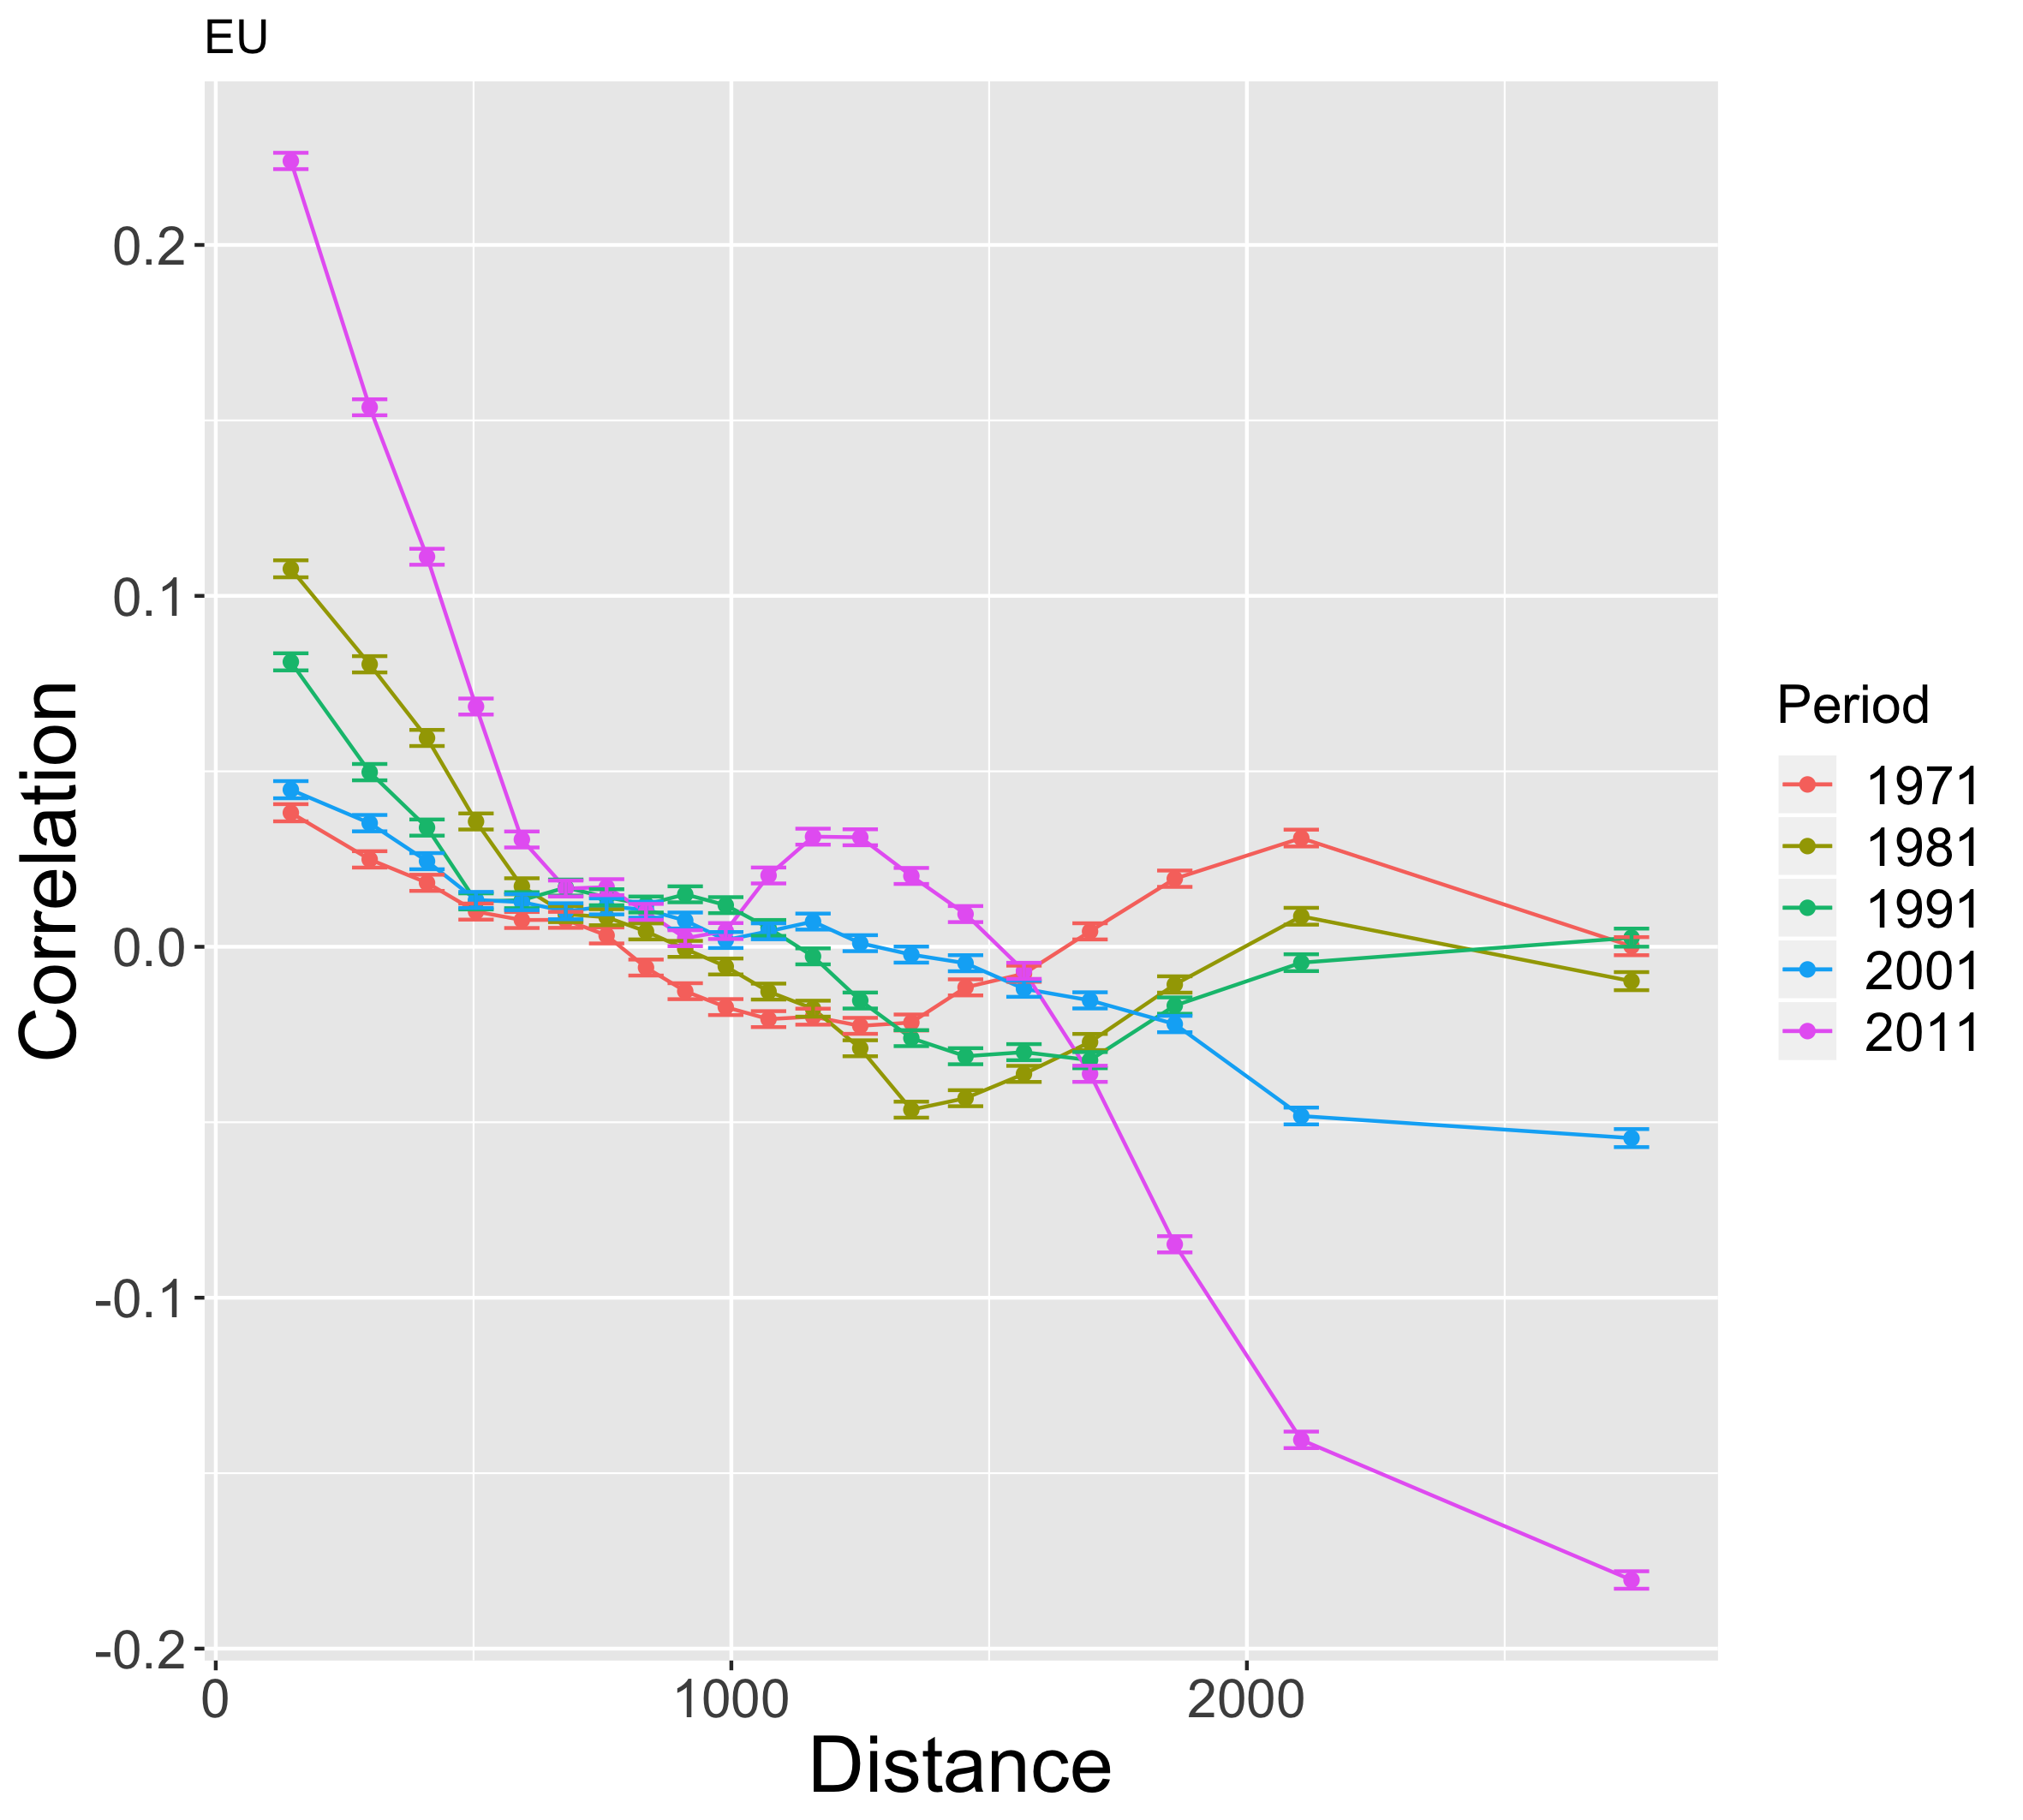
\includegraphics[width=0.48\textwidth]{figures/corrsdist_EU_quantiles21_periods5.png}
\caption{Growth rate correlations as a function of distance between urban areas, for the European urban system.}
\label{fig:empcorrs}
\end{figure}




\section{Multi-scalar model}


The generic multi-scalar model is based on a coupling of several instances of local urban morphogenesis models, and more particularly the reaction-diffusion model studied by \cite{raimbault2018calibration}, through a macroscopic model of interaction between these areas in the spirit of \cite{raimbault2018indirect}. It is therefore able to (i) integrate long range interactions in systems of cities and (ii) simulate the local urban form.

We assume model ontologies similar to the original ones and operate the coupling through a potential dependency of parameters between scales. Let the index $\mu$ denote the macro scale and $M$ the meso scale. Then we assume the parameters of reaction-diffusion instances to depend on time and the macro-scale: $(\alpha,\beta,N_G/P_m)\left[t,\mu\right]$ and similarly for the parameters of the interaction model $(g_0,\vec{gamma},d_G)\left[t,M\right]$.
% TODO Note : here a clarification is needed : shouldnt the macro ontology be a bit modified to include short range and long range interactions ? then cannot be fully generic ? 

We are interested in the following coupling specifications: weak coupling $\mu \rightarrow M$ (no upward causation, study of the consequence on local form of global dynamics), weak coupling $M \rightarrow \mu$ (no downward causation, aggregation of macro trajectories based on macro dynamics to e.g. study their performance compared to the model alone) and strong coupling $M \leftrightarrow \mu$ which can implemented in different ways, but which implies upward and downward causations. The comparison between these coupling is in itself an important knowledge.

We propose the following specification for the strong coupling. At a time step of the macro level $\Delta t_{\mu}$:
\begin{itemize}
	\item Macro level interaction model is computed and population variations $\Delta P_i$ are obtained
	\item Meso level sprawl is simulated in the interval for each area, given this increase. Parameters are fixed by a baseline value but modified as a function of $\Delta P_i$ following simple rules % TODO
	\item The resulting urban form is used to compute an endogenous activity (still with very simple stylized rules) which modifies the macro parameters for each area (these depend then on $i$: $d_G^{(i)},g_0^{(i)}$
\end{itemize}






\begin{figure}[htp]
\centering
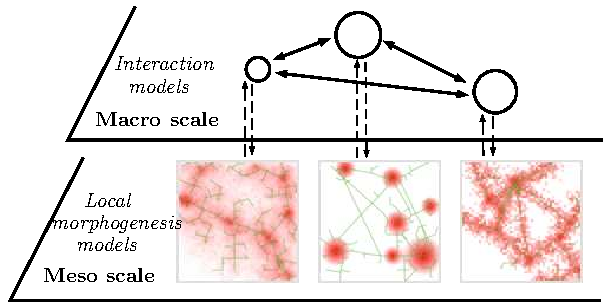
\includegraphics[width=0.48\textwidth]{figures/multiscale_morph.pdf}
\caption{Theoretical flowchart of the multi-scalar model.}
\label{fig:model}
\end{figure}


The model is implemented in scala for performance purposes and an easier integration into the model exploration software OpenMOLE \cite{reuillon2013openmole}.



\section{Discussion}



%\section*{Acknowledgements}
%The research for this work was supported, in part, by the Natural
%Sciences and Engineering Research Council of Canada.

\footnotesize

% Bibliography----------------------------------------------------------------

\bibliographystyle{unsrt}
\bibliography{biblio.bib}



\end{document}
% ----------------------------------------------------------------
